\section{Introduction}

The $n$-queens problem, a combinatorial search problem, concerns the non-attacking (horizontally, vertically, and diagonally) placement of $n$ queens on a $n\times n$ chessboard. The $n$-queens and similar Constraint Satisfaction Problems (CSPs) are classical examples of the limitations of simple backtracking search, with an exponential worst case time complexity that renders solving for large $n$ impractical \citep{sosic90, backtracking}. Although many efficient heuristics have already been proposed for this problem \citep{sosic91, hu03, aima, engel07, agarwal12}, it still is a popular test bed for new Artificial Intelligence (AI) search problem methods. Whilst a toy problem per se, it has found some practical applications such as VLSI routing and testing, data compression, maximum full range communication and parallel optical computing \citep{sosic91, hu03}.

This problem has (at least) two variants depending on the desired number of solutions. A single solution can actually be found trivially without search, since explicit solutions exist $\forall \ n \ge 4$ \citep{trivial}. On the other hand, finding all possible solutions is non-trivial. In this project we will focus on the former variant, implementing and comparing the performance of three different search algorithms: a backtracking method and two local search algorithms. We will first describe the problem mathematically and define the performance indicators for our comparison. In Section \ref{sec:methods} we will describe the implemented algorithms, and we will subsequently illustrate and discuss their performance.

\section{Problem Formulation}

\subsection{Mathematical Model}

A naive formulation would allow any arrangement on the chessboard, resulting in a huge number of combinations (e.g. 3 $\times 10^{14}$ for $n=8$). To reduce the state space, we distribute them so that each column contains only one queen. This restriction ensures that there will be no vertical conflicts, resulting in just 2057 candidate solutions (for $n=8$) \citep{aima}.

Therefore, let array $C=(c_1,...,c_n : c_i \in \{1,...,n\} \ \forall i \in \{1,...,n\})$ be an $n$-queens placement, where $i$ is the column number, and $c_i$ is the row number of the $i$-th queen. To ensure that we have no horizontal or diagonal collisions, we need two more constraint equations. The first constraint is expressed as $c_i\ne c_j, \ \forall i \ne j$, namely no pairs of columns should be in the same row. The second constraint can be expressed as $|i-j| \ne |c_i - c_j|, \ \forall i \ne j$, namely no pair can be in the same diagonal.

Having defined the constraint and state representation formulas, the objective function that returns the total amount of direct and indirect collisions of $C$ is given by:
\smallskip
\begin{align}
\label{eq:1}
n_c(C) &= \sum_{i=1}^{n-1} \sum_{j=i+1}^n f(c_i,c_j) \\
\label{eq:2}
f(c_i, c_j) &=  
\begin{cases}
   1, & c_i = c_j \\
   1, & |i-j| = |c_i - c_j| \\
    0,              & \text{otherwise}
\end{cases}
\end{align}

We notice that a brute-force approach in calculating the total amount of direct and indirect conflicts using Equation (\ref{eq:1}) would require $O(n^2)$ operations. However, a better approach has been formulated in \citet{sosic91}. Based on their work, we define the additional data structures: 1) an array $D_{\text{neg}}$ containing the total number of queens per negative diagonal $D_{\text{neg}}=(d_{\text{neg},1},...,d_{\text{neg},2n-1} : d_{i} \in \{0,...,n\} \ \forall i \in \{1,...,2n-1\})$, 2) a similarly defined array $D_{\text{pos}}$ for the positive diagonals, 3) an array $R=(r_{1},...,r_{n} : r_{i} \in \{0,...,n\} \ \forall i \in \{1,...,n\})$ containing the total number of queens per row, and 4) an array $Q=(q_1,...,q_n : q_i \in \{0, 1\} \ \forall i \in \{1,...,n\})$ denoting whether a queen is attacked (1) or not (0).

Note that each queen belongs to a column $i$, a row $c_i$, a negative diagonal $i-c_{i}+n$ and a positive diagonal $i+c_{i}-1$. Given the description above, we can now denote an $O(n)$ function for the number of \emph{direct only} conflicts as:
\smallskip
\begin{align}
\label{eq:3}
n_c(D_{\text{neg}}, D_{\text{pos}}, R) = \sum_{i=1}^{2n-1}(d_{\text{neg,i}} - \text{min}(1, d_{\text{neg,i}}) + d_{\text{pos,i}} - \text{min}(1, d_{\text{pos,i}})) + \sum_{i=1}^{n}(r_i - \text{min}(1, r_i))
\end{align}

\subsection{Performance Indicators}

In order to assess the quality of our methods, we will employ three different performance indicators: 1) average execution time, 2) average memory used, and 3) average number of operations. Time and memory measurements will give an estimate of the time and space complexity of each method respectively. However, absolute time is hardware-dependent, and may even vary in the same machine due to other operating system processes. Hence, the average number of operations offers a hardware and software-independent time metric. See the next section for how operations and memory usage are estimated.


\section{Methods}
\label{sec:methods}

We selected three algorithms to implement in MATLAB: 1) forward checking with minimum remaining values (FC-MRV) algorithm as a CSP solver \citep{aima}, 2) the min-conflict algorithm as a CSP/local search method  \citep{aima}, and 3) QS2, a swapping local search algorithm \citep{sosic91}. We chose these algorithms since previous results have illustrated their good performance, especially in comparison to simpler backtracking-based methods \citep{aima, sosic91}. For the exact code implementation, please refer to the accompanying source code.

\subsection{FC-MRV Algorithm}

Algorithm \ref{alg:fc-mrv} contains the pseudo-code of our FC-MRV recursive implementation in MATLAB. The initial call is performed by Algorithm\ref{alg:fc-mrv-main}. The successor state is determined by the recursive calls of FC-MRV. More specifically, the MRV method (line 8) chooses the unassigned column with the minimum number of remaining valid rows (choosing randomly if there are multiple). All valid rows are then checked one-by-one in lines 9-14. For each row, a new recursive call updates the current domain of the remaining unassigned columns (lines 1-5). The current domain is stored in a $n\times n$ matrix, which represents the board and contains 1 for valid positions and 0 for invalid ones. This cycle of recursions continues until either a complete solution is found, or until a column does not have any remaining valid positions left (which means that the previously selected row is not part of a valid configuration).

\textbf{Performance Estimation:} In order to estimate the number of operations and the memory used we make the following assumptions: 1) Each call of find(), UpdateDomain(), MRV() and initialization of solution array $C$ costs $n$ operations. 2) Initialization of current domain matrix costs $n^2$ operations. 3) Current domain matrix costs $n^2$ arbitrary memory units, which is replicated for each recursive call. 4) Each recursion keeps two solution arrays (the old and new one) costing $2n$. 5) An array that keeps the unassigned queens costs $n$.

\begin{algorithm}
\caption{FC-MRV(currDomain, solution, row, column)}\label{alg:fc-mrv}
\begin{algorithmic}[1]
\ForAll{i : unassigned columns}
\State UpdateDomain(currDomain, row, column, i) using Equation \ref{eq:2}
\If{no available rows left for column i}
return empty solution
\EndIf
\EndFor
\If{all columns have been assigned with a row}
return solution
\EndIf
\State newColumn = MRV(currDomain, solution)
\ForAll{newRow : available rows for newColumn}
\State solution[newColumn] = newRow
\State newSolution = FC-MRV(currDomain, solution, newRow, newColumn) 
\If{newSolution not empty}
return newSolution
\EndIf
\EndFor
\State return empty solution
\end{algorithmic}
\end{algorithm}

\begin{algorithm}
\caption{FC-MRV-MAIN(n)}\label{alg:fc-mrv-main}
\begin{algorithmic}[1]
\State Initialize empty solution
\State Initialize currDomain $ = \boldsymbol{1}^{n\times n}$
\State Choose a random column j
\ForAll{i : rows}
\State solution[j] = i
\State newSolution = FC-MRV(currDomain, solution, i, j) 
\If{newSolution not empty}
return newSolution
\EndIf
\EndFor
\end{algorithmic}
\end{algorithm}

%\begin{algorithm}
%\caption{UpdateDomain(currDomain, $q_i$, $i$, $j$)}\label{alg:UpdateDomain}
%\begin{algorithmic}[1]
%\ForAll{$q_j$ : rows}
%\If{$c(q_i, q_j)==1$}
%currDomain[$i$,$j$] = 0
%\EndIf
%\EndFor
%\end{algorithmic}
%\end{algorithm}

\subsection{Min-Conflicts Algorithm}

Algorithm \ref{alg:min-conflicts} contains the pseudo-code of our min-conflicts implementation in MATLAB. The successor operations of this method are in lines 14-15, where local changes upon the current state happen by randomly choosing an attacked queen and moving her to the row with the lowest number of conflicts. The above procedure is repeated until a maximum number of steps is reached or a solution is found. The outer while loop guarantees completeness.

\textbf{Performance Estimation:} In order to estimate the number of operations and the memory used we make the following assumptions: 1) Each call of checkDiagonals(), countDiagConflicts(), findAttackedQueens(), find(), min() and randperm() cost $n$ operations. 2) Initialization of $R$ and array that keeps conflicts per row (line 12) cost $n$ operations. 3) $D_{\text{pos}}$ and $D_{\text{neg}}$ cost $2n$ arbitrary memory units, whereas the rest of the arrays cost $n$ units. With these assumptions the space complexity is linear, estimated as $9n$.

\begin{algorithm}
\caption{MIN-CONFLICTS(n)}\label{alg:min-conflicts}
\begin{algorithmic}[1]
\State Set a random permutation as initial solution $C$
\State Calculate $D_{\text{pos}}$, $D_{\text{neg}}$ and $R$ for initial solution
\State Calculate $n_c$ using Equation \ref{eq:3}
\State Calculate attacked queens in $Q$
\State steps = 0
\State Define constants maxSteps
\While{$n_c > 0$} 
\While{steps $<$ maxSteps}
\State steps++
\State Choose an attacked Queen i randomly
\ForAll{row : 1 to $n$}
\State Calculate conflicts per row
\EndFor
\State Choose the row that minimizes the conflicts (choose randomly if there are more than one)
\State Perform change updating $C$, $D_{\text{pos}}$, $D_{\text{neg}}$ and $R$
\If{$n_c = 0$}
\State return solution $C$
\Else
\State Recalculate attacked queens in $Q$
\EndIf
\EndWhile
\State Set a random permutation as initial solution $C$
\State Calculate $D_{\text{pos}}$, $D_{\text{neg}}$ and $R$ for initial solution
\State Calculate $n_c$ using Equation \ref{eq:3}
\State Calculate attacked queens in $Q$
\State steps = 0
\EndWhile
\end{algorithmic}
\end{algorithm}

\newpage
\subsection{QS2: Swapping Queens}

Algorithm \ref{alg:swap} contains the pseudo-code of our min-conflicts implementation in MATLAB. The successor operations take place in lines 13-14. For each attacked queen, we randomly choose another queen and we check whether swapping their rows will decrease $n_c$. If it does, then the state is updated, performing the swap. The limit of line 18 is used as a way of preventing breaking the for loop prematurely and recalculating the attacked queens unnecessarily \citep{sosic91}. Again the outer while loop guarantees that an optimal solution will be returned.

\textbf{Performance Estimation:} In order to estimate the number of operations and the memory used we make the following assumptions: 1) Each call of checkDiagonals(), countDiagConflicts(), findAttackedQueens(), find(), randperm() cost $n$ operations. 2) For each iteration of for loop in line 10, we add a single operation. 3) $D_{\text{pos}}$ and $D_{\text{neg}}$ cost $2n$ arbitrary memory units, whereas the rest of the arrays cost $n$ units. With these assumptions the space complexity is linear,  estimated as $7n$.

\begin{algorithm}
\caption{QS2(n)}\label{alg:swap}
\begin{algorithmic}[1]
\State Set a random permutation as initial solution $C$
\State Calculate $D_{\text{pos}}$ and $D_{\text{neg}}$ for initial solution
\State Calculate $n_c$ using Equation \ref{eq:3}
\State Calculate attacked queens in $Q$
\State steps = 0
\State Define constants maxSteps and C1
\State limit = C1 $\times n_c$ 
\While{$n_c > 0$} 
\While{steps $<$ maxSteps}
\ForAll{i : attacked Queens}
\State steps++
\State Choose another column j
\If{swapping rows between column i and column j decreases conflicts}
\State{Perform swap updating $C$, $D_{\text{pos}}$ and $D_{\text{neg}}$}
\If{$n_c = 0$}
\State return solution $C$
\Else
\If{$n_c < $ limit}
\State limit = C1 $\times n_c$ 
\State Recalculate attacked queens in $Q$
\State Break loop
\EndIf
\EndIf
\EndIf
\EndFor
\EndWhile
\State Set a random permutation as initial solution $C$
\State Calculate $D_{\text{pos}}$ and $D_{\text{neg}}$ for initial solution
\State Calculate $n_c$ using Equation \ref{eq:3}
\State Calculate attacked queens in $Q$
\State steps = 0
\State limit = C1 $\times n_c$ 
\EndWhile
\end{algorithmic}
\end{algorithm}

\section{Results}

Table \ref{table:execution-time} contains the real execution time of our algorithms for various number of queens, whereas Figure \ref{fig:execution-time} depicts the same results graphically. The results clearly show that FC-MRV approximates an exponential time complexity, which is the theoretical worst case time complexity of backtracking-based methods \citep{aima}. On the other hand, the min-conflicts and QS2 algorithms run in polynomial time, exhibiting a significantly better performance than FC-MRV for $n \ge 60$ queens. For a small number of queens, QS2 shows a worse temporal performance, probably because its time complexity constants dominate its running time. Nevertheless, the swapping mechanism of QS2 clearly outperforms the min-conflicts search for many queens.  Similar curves can be seen in Table \ref{table:operations} and Figure \ref{fig:operations}, where the average number of operations are depicted.

Finally, Table \ref{table:space} and Figure \ref{fig:space} contain our estimated measurements of each algorithm's memory usage. Again, min-conflicts and QS2 obviously have a linear space complexity (as expected from local search algorithms), since they only need to store the arrays $C$, $D_{\text{pos}}$, $D_{\text{neg}}$, $R$ and $Q$, whose length linearly depends  on $n$. In contrast, FC-MRV exhibits a huge space cost, even for smaller problem sizes, due to the rapidly increasing number of recursive calls.

\begin{figure}[htpb]
\centering
\makebox[\textwidth]{%
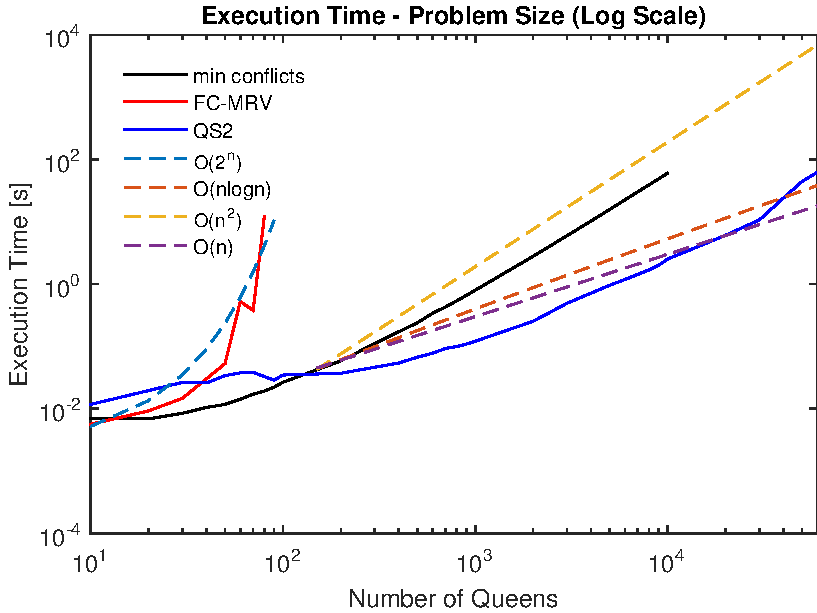
\includegraphics[width=0.8\textwidth, angle = 0, trim = 0mm 0mm 0mm 0mm,clip=true]{images/execution-time.pdf}}
\caption{Real execution time as a function of $n$ from the data of Table \ref{table:execution-time}. To reveal the scaling of each algorithm's time complexity, we also draw representative exponential and polynomial functions.}
\label{fig:execution-time}
% Place the label just after the caption to make the link work
\end{figure} % table makes a floating object with a title

\begin{figure}[htpb]
\centering
\makebox[\textwidth]{%
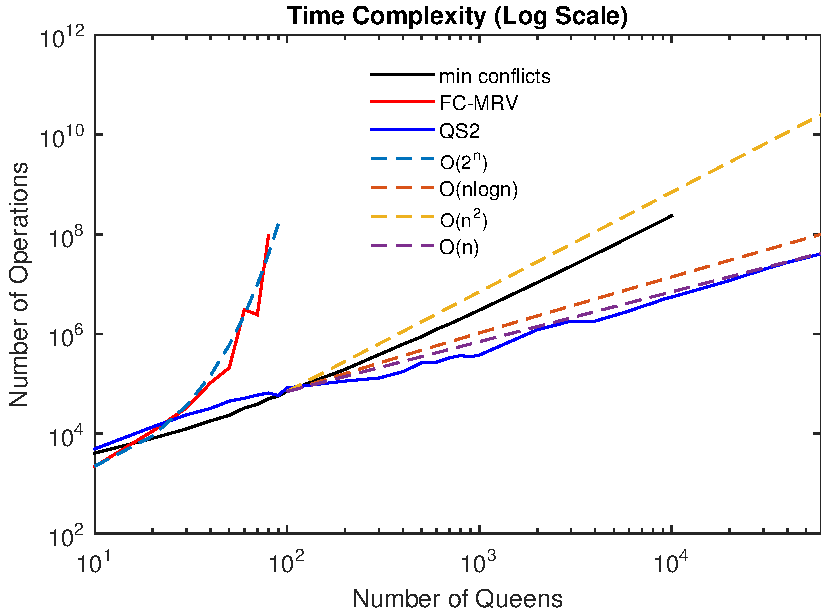
\includegraphics[width=0.8\textwidth, angle = 0, trim = 0mm 0mm 0mm 0mm,clip=true]{images/time-complexity.pdf}}
\caption{Number of operations as a function of $n$ from the data of Table \ref{table:operations}. To reveal the scaling of each algorithm's time complexity, we also draw representative exponential and polynomial functions.}
\label{fig:operations}
% Place the label just after the caption to make the link work
\end{figure} % table makes a floating object with a title

\begin{figure}[htpb]
\centering
\makebox[\textwidth]{%
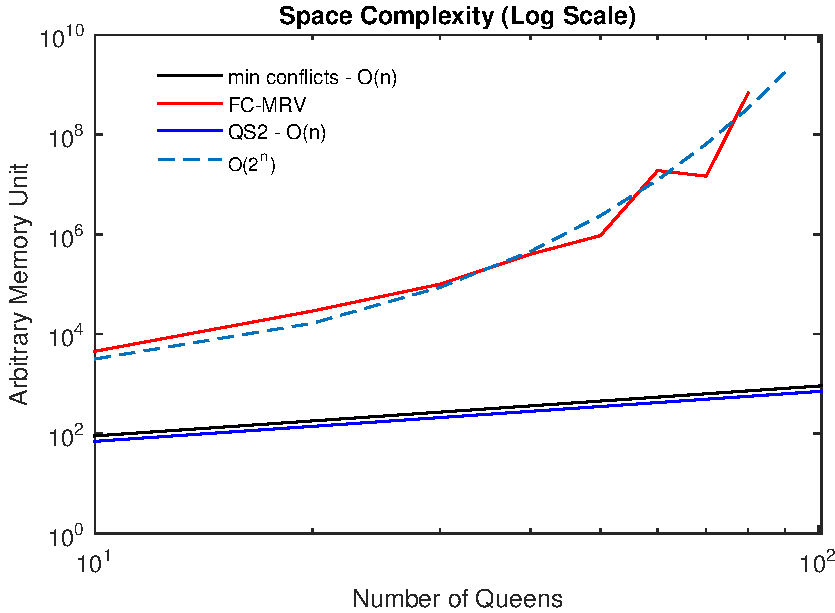
\includegraphics[width=0.8\textwidth, angle = 0, trim = 0mm 0mm 0mm 0mm,clip=true]{images/space-complexity.pdf}}
\caption{Memory usage as a function of $n$ from the data of Table \ref{table:space}. To reveal the scaling of FC-MRV we also draw a representative exponential function. The min-conflicts and QS2 curves are linear as explained in Section \ref{sec:methods}.}
\label{fig:space}
% Place the label just after the caption to make the link work
\end{figure} % table makes a floating object with a title

\begin{figure}[htpb]
\centering
\makebox[\textwidth]{%
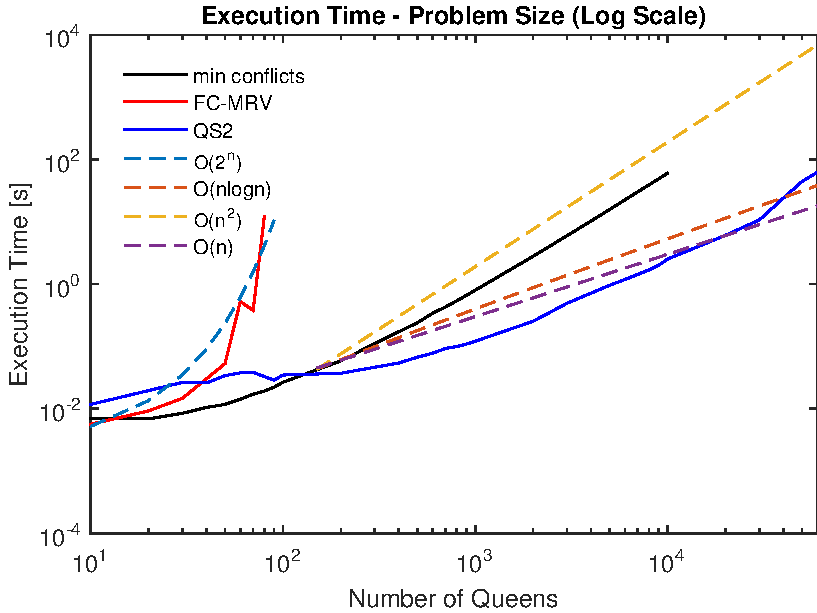
\includegraphics[width=0.8\textwidth, angle = 0, trim = 0mm 0mm 0mm 0mm,clip=true]{images/execution-time.pdf}}
\caption{Real execution time as a function of $n$ from the data of Table \ref{table:execution-time}. To reveal the scaling of each algorithm's time complexity, we also draw representative exponential and polynomial functions.}
\label{fig:execution-time}
% Place the label just after the caption to make the link work
\end{figure} % table makes a floating object with a title

\begin{figure}[htpb]
\centering
\makebox[\textwidth]{%
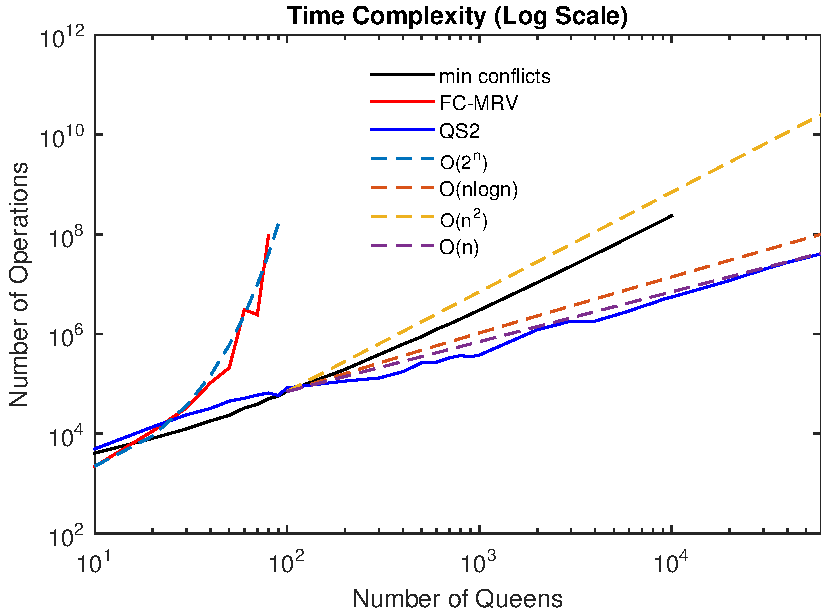
\includegraphics[width=0.8\textwidth, angle = 0, trim = 0mm 0mm 0mm 0mm,clip=true]{images/time-complexity.pdf}}
\caption{Number of operations as a function of $n$ from the data of Table \ref{table:operations}. To reveal the scaling of each algorithm's time complexity, we also draw representative exponential and polynomial functions.}
\label{fig:operations}
% Place the label just after the caption to make the link work
\end{figure} % table makes a floating object with a title

\begin{figure}[htpb]
\centering
\makebox[\textwidth]{%
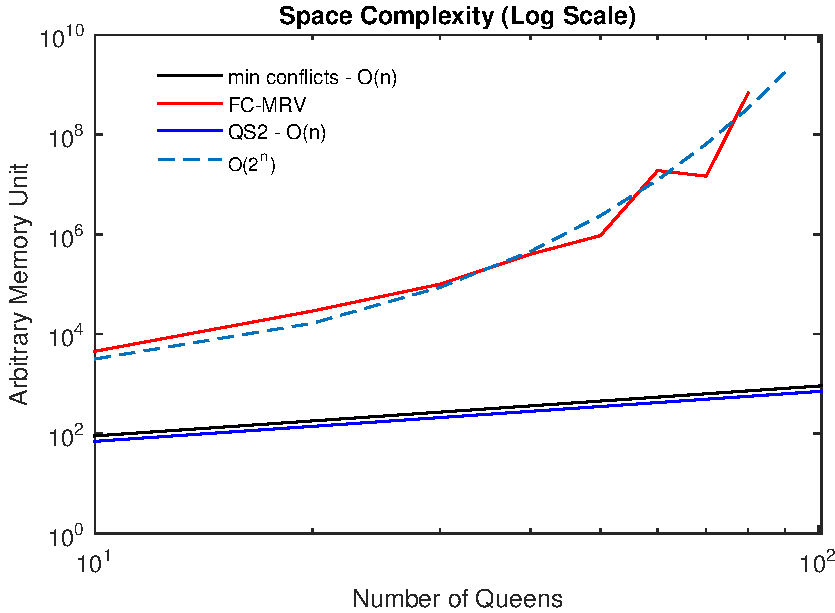
\includegraphics[width=0.8\textwidth, angle = 0, trim = 0mm 0mm 0mm 0mm,clip=true]{images/space-complexity.pdf}}
\caption{Memory usage as a function of $n$ from the data of Table \ref{table:space}. To reveal the scaling of FC-MRV we also draw a representative exponential function. The min-conflicts and QS2 curves are linear as explained in Section \ref{sec:methods}.}
\label{fig:space}
% Place the label just after the caption to make the link work
\end{figure} % table makes a floating object with a title

\section{Conclusions}

In this report we implemented in MATLAB three different methods for solving the $n$-queens problem. Our results clearly illustrated the superior performance of two local search algorithms (min-conflicts and QS2) against a typical backtracking-based method (FC-MRV). Both local search algorithms started from a random state, ensuring that no two queens can be found in the same column and row. A better initialization may have been a partial queen placement with no conflicts as shown in \citet{sosic91}. Finally, more general methods, such as bioinspired algorithms and neural networks, can also be used with success \citep{review}.











